\documentclass{beamer}

\documentclass{beamer}
\usepackage[utf8]{inputenc}
\usepackage[ngerman]{babel}
\usepackage{url}
\usepackage{xcolor}

\usetheme[compress]{Berlin}
\setbeamerfont{headline}{size=\large}
\setbeamerfont*{section in head/foot}{size=\tiny}
\setbeamertemplate{toc}{circle}
\setbeamertemplate{itemize subitem}[triangle] % if you want a triangle
\setbeamercovered{transparent}

\definecolor{myBlue}{rgb}{0,0.55,0.8}
\usecolortheme[named=myBlue]{structure}

\title{Das \LaTeX-KBS}
\subtitle{\small Grundlagen von \LaTeX, Ti\textit{k}Z und Co.}
\author
{
	Walter Stieben \texttt{\href{mailto:4stieben@informatik.uni-hamburg.de}{4stieben@inf}}\\
	\href{http://hauke-stieler.de/}{Hauke Stieler} \texttt{\href{mailto:4stieler@informatik.uni-hamburg.de}{4stieler@inf}}
}
\date{\footnotesize 12.01.2016}

\begin{document}
	\maketitle
	\tableofcontents\newpage
	\section{Was ist \TeX{} und \LaTeX{}}
		\subsection*{asd}
		\begin{frame}{Was ist \LaTeX{}}
			\textbf{\LaTeX{} und \TeX{}:}
			\begin{itemize}
				\item \TeX{} ist ein Textsatzsystem von Donald E. Knuth
				\item \LaTeX{} ist ein Satz von Makros für \TeX
				\item WYSIWYT (What You See Is What You Type)
			\end{itemize}
			\vspace{0.2cm}
			\textbf{Vorteile von \LaTeX{}:}
			\begin{itemize}
				\item Ergebnis sieht hübsch aus
				\item \LaTeX{} kümmert sich um die Formatierung
				\item Der Quelltext lässt sich Versionsverwalten
				\item Für mathematische Formeln sehr gut
				\item ``Ich möchte X mit \LaTeX{} machen'' $\rightarrow$
				Suchmaschine: ``latex X'' eingeben $\rightarrow$
				Ergebnis in den Quelltext kopieren
			\end{itemize}
		\end{frame}
\end{document}

\title{Das \LaTeX-KBS}
\subtitle{\small Grundlagen von \LaTeX, Beamer und Tipps für Hausaufgaben, Seminararbeiten, etc.}
\author
{
	Walter Stieben \texttt{\href{mailto:4stieben@informatik.uni-hamburg.de}{4stieben@inf}}\\
	\href{http://hauke-stieler.de/}{Hauke Stieler} \texttt{\href{mailto:4stieler@informatik.uni-hamburg.de}{4stieler@inf}}\\
  Ruben Felgenhauer \texttt{\href{mailto:4felgenh@informatik.uni-hamburg.de}{4felgenh@inf}}
}

\date{\footnotesize \today}

\begin{document}
	\maketitle
		
	%%%%%%%%%%%%%%%%%%%%%%%%%%%%%%%%%%%%%%%%%%%%%%%%%%%%%%%%%%%%%%%%%%%%%%%
		
	\begin{frame}
		\begin{center}
			Danke Henning (\texttt{8pridoeh}) dass wir deine Folien aus dem WS14/15 benutzen dürfen :D
		\end{center}
	\end{frame}
		
	%%%%%%%%%%%%%%%%%%%%%%%%%%%%%%%%%%%%%%%%%%%%%%%%%%%%%%%%%%%%%%%%%%%%%%%
		
	\begin{frame}
		\begin{minipage}[0.5\textheight]{0.5\textwidth}
			\tableofcontents[hideallsubsections]
		\end{minipage}
		\begin{minipage}{0.45\textwidth}
			
\includegraphics[width=1.05\textwidth]{./images/gib-word-keine-chance}
		\end{minipage}
	\end{frame}
		
	%%%%%%%%%%%%%%%%%%%%%%%%%%%%%%%%%%%%%%%%%%%%%%%%%%%%%%%%%%%%%%%%%%%%%%%
		
	\section{Was ist \LaTeX{}}
		\subsection{Einführung}
		\begin{frame}{Was ist \LaTeX{}}
			\slideheading{\LaTeX{} und \TeX{}:}
			\begin{itemize}
				\item \TeX{} ist ein Textsatzsystem von Donald E. Knuth
				\item \LaTeX{} ist ein Satz von Makros für \TeX
				\item WYSIWYM (What You See Is What You Mean)
			\end{itemize}
			\vspace{0.1cm}
			\slideheading{Vorteile von \LaTeX{}:}
			\begin{itemize}
				\item Ergebnis sieht hübsch aus
				\item \LaTeX{} kümmert sich um die Formatierung
				\item Der Quelltext lässt sich Versionsverwalten
				\item Für mathematische Formeln sehr gut
				\item ``Ich möchte X mit \LaTeX{} machen'' $\rightarrow$
				Suchmaschine: ``latex X'' eingeben $\rightarrow$
				Ergebnis in den Quelltext kopieren
				\item Der meiste Code ist wiederverwendbar
			\end{itemize}
		\end{frame}
		
		%%%%%%%%%%%%%%%%%%%%%%%%%%%%%%%%%%%%%%%%%%%%%%%%%%%%%%%%%%%%%%%%%%%%%%%
		\subsection{\LaTeX{} installieren}
		\begin{frame}{\LaTeX-Distribution}
%			\slideheading{\LaTeX-Distribution:}
Die \LaTeX-Distribution stellt eine Sammlung von Paketen und Programmen zum Kompilieren bereit (Backend). \\
			\begin{description}
				\item[GNU/Linux] Nutzt den Paketmanager eurer Distribution. Debian/Ubuntu: \texttt{apt-get install texlive} \\
				oder \texttt{apt-get install texlive-full} (\(>\) 2 GB)
				\item[Windows] MiKTeX  oder TeX Live herunterladen und installieren. \url{http://miktex.org/} \url{http://www.tug.org/texlive/}
				\item[Mac OS] MacTex herunterladen und installieren. \url{http://tug.org/mactex/} 
			\end{description}
			\end{frame}	
			
			
		\begin{frame}{\LaTeX-Editoren}
%			\slideheading{\LaTeX-Editoren:}
			\begin{description}
				\item[Kile] Guter Editor für GNU/Linux (KDE).
				\item[Gummi] Editor für GNU/Linux (GTK) mit Live-Preview
				\item[AUCTeX] für Emacs-Benutzer
				\item[Texmaker] Editor für alle Betriebssysteme
				\item[Texstudio] Fork von Texmaker mit mehr Funktionen
			\end{description}
			 und viele mehr \dots
		\end{frame}
		
		%%%%%%%%%%%%%%%%%%%%%%%%%%%%%%%%%%%%%%%%%%%%%%%%%%%%%%%%%%%%%%%%%%%%%%%
		
		\begin{frame}{Overleaf}
			Online Editor mit Live-Preview (\url{https://www.overleaf.com})
			
			\begin{center}
				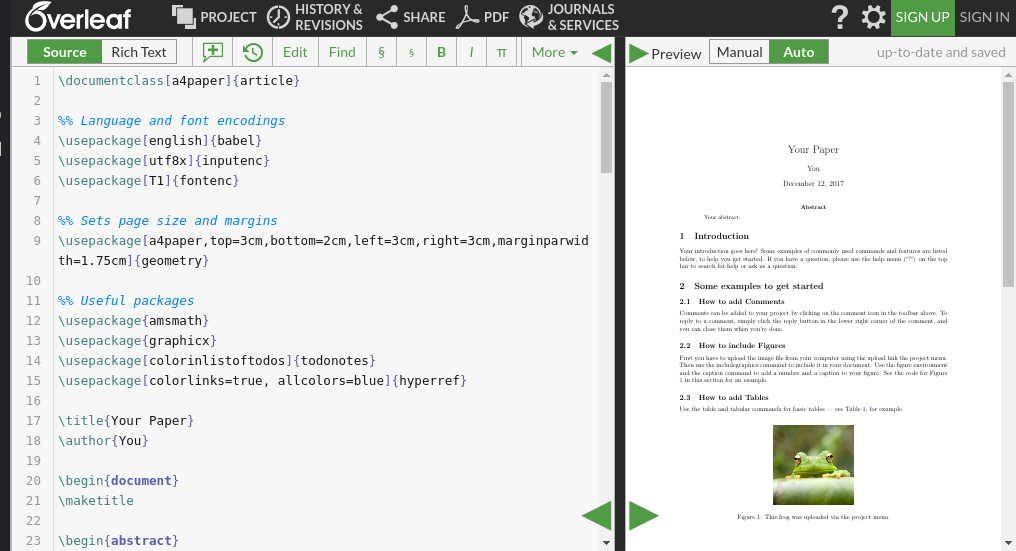
\includegraphics[width=0.75\textwidth]{images/overleaf}
			\end{center}
		\end{frame}
		
		%%%%%%%%%%%%%%%%%%%%%%%%%%%%%%%%%%%%%%%%%%%%%%%%%%%%%%%%%%%%%%%%%%%%%%%
		
		\begin{frame}{Verschiedene \LaTeX{}-Compiler}
			Es gibt verschiedenen Compiler für \LaTeX{}. Heute: \textbf{pdflatex}
			\slideheading{Vorteile von pdflatex:}
			\begin{itemize}
				\item Direktes erzeugen einer PDF
				\item Viele PDF-Features nutzbar
				\item Einfach zu verwenden
			\end{itemize}
			\slideheading{Nachteile von pdflatex:}
			\begin{itemize}
				\item Kein \texttt{pstricks} nutzbar.
				\item Postscript-Dateien nicht direkt einbindbar
				\item Keine vollständige Unicode-Unterstützung (wie Xe\LaTeX)
			\end{itemize}
		\end{frame}
		
		%%%%%%%%%%%%%%%%%%%%%%%%%%%%%%%%%%%%%%%%%%%%%%%%%%%%%%%%%%%%%%%%%%%%%%%
		
		\begin{frame}{Detexify -- \LaTeX-Symbolerkennung}
		\begin{minipage}[0.5\textheight]{0.5\textwidth}
			\begin{center}
			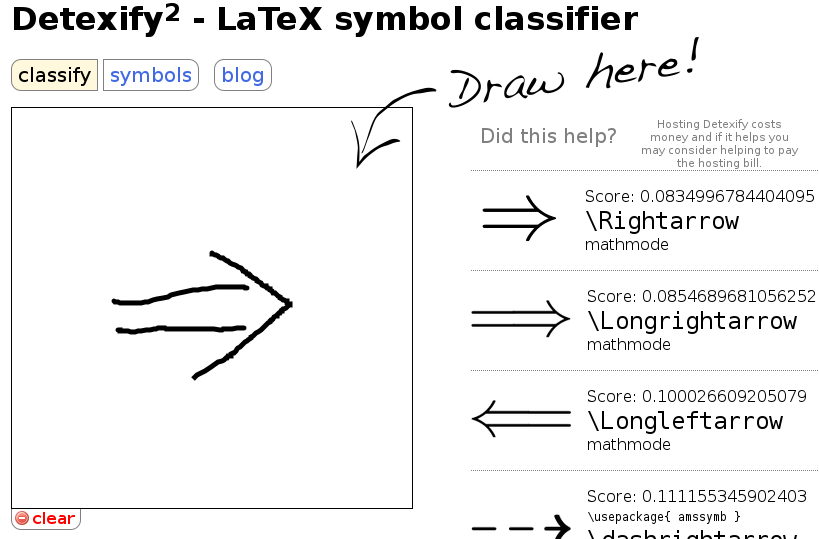
\includegraphics[height=0.48\textheight]{images/detexify}
			\vspace{0.5cm}
			\Large \href{http://detexify.kirelabs.org/}{detexify.kirelabs.org}
			\end{center}
		\end{minipage}
		\begin{minipage}{0.45\textwidth}
			\begin{center}
			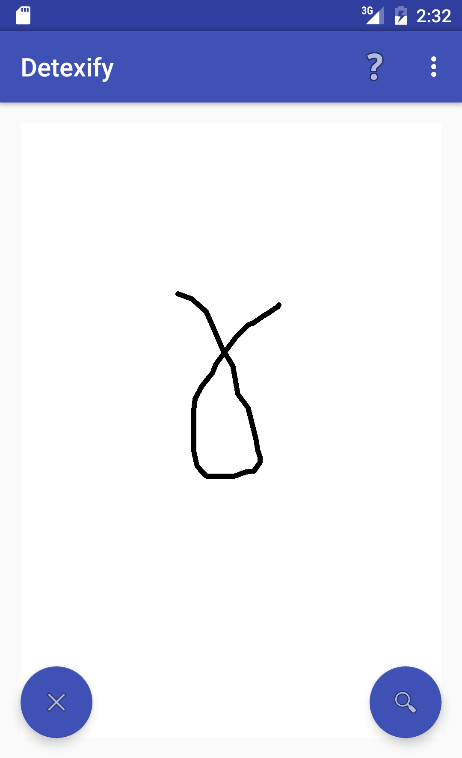
\includegraphics[height=0.48\textheight]{images/detexify-app1}
			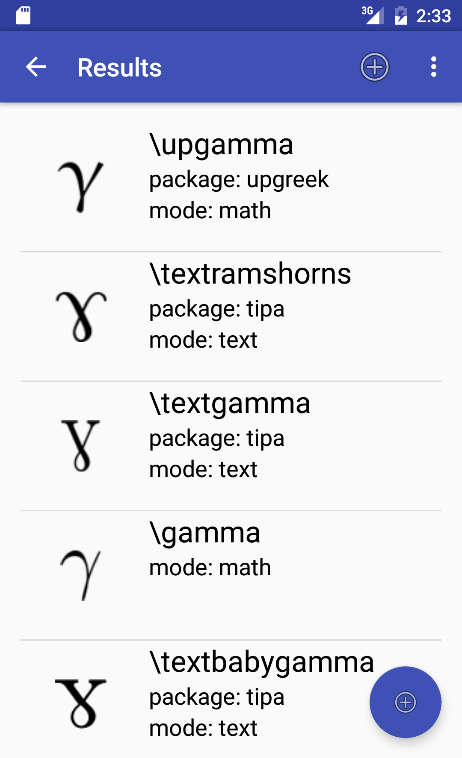
\includegraphics[height=0.48\textheight]{images/detexify-app2}
			\vspace{0.5cm}
			\Large \href{https://play.google.com/store/apps/details?id=website.marty.detexify}{Detexify im Play Store}
			\end{center}
		\end{minipage}
				
		\end{frame}

		
		%%%%%%%%%%%%%%%%%%%%%%%%%%%%%%%%%%%%%%%%%%%%%%%%%%%%%%%%%%%%%%%%%%%%%%%
		
		\begin{frame}{Anmerkungen}
			\slideheading{Achtung:} \TeX{} ist eine Programmiersprache! Lasst nur vertrauenswürdige
			Menschen \TeX/\LaTeX-Code auf eurem Rechner/Server ausführen.
			
			\vspace{0.2cm}
			\slideheading{Anmerkung:} Man kann \textbf{\url{https://www.overleaf.com}} zum live-nachcoden benutzen.
		\end{frame}
		
		%%%%%%%%%%%%%%%%%%%%%%%%%%%%%%%%%%%%%%%%%%%%%%%%%%%%%%%%%%%%%%%%%%%%%%%
		
		\section{Grundlagen von \LaTeX{} und \TeX}
		\subsection{Theorie}
		
		\begin{frame}{Dokumentenklassen}
			\begin{itemize}
				\item Die Dokumentenklasse beschreibt wie ein Dokument aussieht
				\item Ihr beschreibt was ihr schreibt (z.\,B. was eine Überschrift ist)
				\item \LaTeX{} formatiert euer Dokument mit Hilfe der Dokumentenklasse, \textbf{nicht ihr}!
			\end{itemize}
			\vspace{0.1cm}
			\slideheading{Beispiele für Dokumentenklassen:}
			\begin{description}
				\item[Scrartcl, article:] Artikel im Umfang von mehreren Seiten
				\item[Scrllr2, letter:] Briefe
				\item[Scrreprt, report:] Reports, Umfang mehr als 15 Seiten
				\item[Scrbook, book:] Bücher
			\end{description}
		\end{frame}
		
		%%%%%%%%%%%%%%%%%%%%%%%%%%%%%%%%%%%%%%%%%%%%%%%%%%%%%%%%%%%%%%%%%%%%%%%
		
		\begin{frame}{Syntax - Befehle und Umgebungen}
			\slideheading{Befehle:}
			\begin{itemize}
				\item Beginnen mit einem Backslash ( \textbackslash... )
				\item Parameter in geschweiften Klammern ( \{...\} )
				\item \textit{Optionale} Parameter in eckigen ( [...] )
				\item Manchmal auch als \texttt{*}-Variante (leicht verändertes Verhalten; s. \texttt{align} und \texttt{align*} Umgebung später)
			\end{itemize}
			\slideheading{Umgebungen:}
			\begin{itemize}
				\item Beginnen mit dem \texttt{\textbackslash begin\{name\}} Befehl
				\item und enden mit dem \texttt{\textbackslash end\{name\}} Befehl
				\item Formatieren ganze Textblöcke
			\end{itemize}
		\end{frame}
		
		%%%%%%%%%%%%%%%%%%%%%%%%%%%%%%%%%%%%%%%%%%%%%%%%%%%%%%%%%%%%%%%%%%%%%%%
		
		\begin{frame}{Aufbau des Dokumentes}
			\slideheading{Dokument:}
			\begin{enumerate}
				\item Dokumentenklasse wählen
				\item Pakete laden
				\item Einstellungen vornehmen, Styles ändern, Befehle definieren, et.
				\item Dokument öffnen
				\item Inhalte schreiben
				\item Dokument schließen
			\end{enumerate}
		\end{frame}
		
		%%%%%%%%%%%%%%%%%%%%%%%%%%%%%%%%%%%%%%%%%%%%%%%%%%%%%%%%%%%%%%%%%%%%%%%
		
		\begin{frame}{Schriftgrößen}
			\slideheading{Schriftgrößen:}\hspace{5mm}
			\begin{tabular}{l l}
				tiny 			& \tiny\textbackslash tiny\normalsize\\
				scriptsize 		& \scriptsize\textbackslash scriptsize\normalsize\\
				footnotesize 	& \footnotesize\textbackslash footnotesize\normalsize\\
				small 			& \small\textbackslash small\normalsize\\
				normalsize 		& \normalsize\textbackslash normalsize\normalsize\\
				large 			& \large\textbackslash large\normalsize\\
				Large 			& \Large\textbackslash Large\normalsize\\
				LARGE 			& \LARGE\textbackslash LARGE\normalsize\\
				huge 			& \huge\textbackslash huge\normalsize\\
				Huge 			& \Huge\textbackslash Huge\normalsize
			\end{tabular}
		\end{frame}
		
		%%%%%%%%%%%%%%%%%%%%%%%%%%%%%%%%%%%%%%%%%%%%%%%%%%%%%%%%%%%%%%%%%%%%%%%
		
		\subsection{Textsatz-Grundlagen}
		
		\begin{frame}[containsverbatim]{Mein erstes Dokument}
			\begin{latexcode}
\documentclass[a4paper,10pt]{scrartcl}
\usepackage[utf8]{inputenc}
\usepackage[T1]{fontenc}
\usepackage[ngerman]{babel}
\usepackage{lmodern}

\author{Max Mustermann}
\title{Mein erstes Dokument}

\begin{document}
	\maketitle
	Hello World!
\end{document}
			\end{latexcode}
			\begin{textblock}{10}(7.5,10.5)
				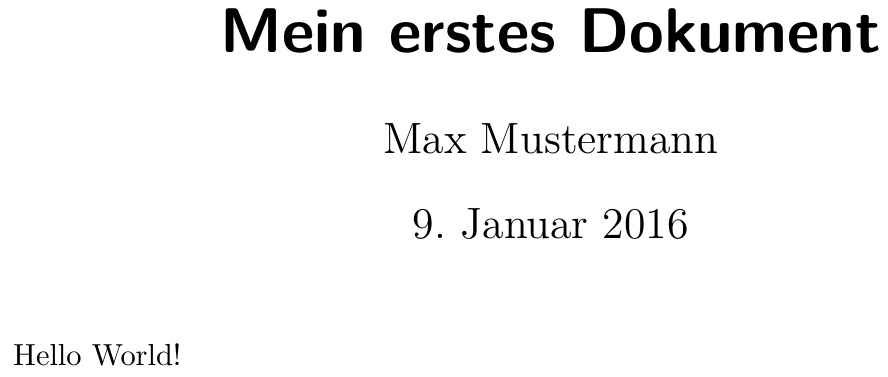
\includegraphics[width=5.5cm]{images/erstes-dokument-scrartcl}
			\end{textblock}
		\end{frame}
		
		%%%%%%%%%%%%%%%%%%%%%%%%%%%%%%%%%%%%%%%%%%%%%%%%%%%%%%%%%%%%%%%%%%%%%%%
		
		\begin{frame}[containsverbatim]{Mein erstes Dokument}
			\begin{latexcode}
\documentclass[a4paper,10pt]{article}
\usepackage[utf8]{inputenc}
\usepackage[T1]{fontenc}
\usepackage[ngerman]{babel}
\usepackage{lmodern}

\author{Max Mustermann}
\title{Mein erstes Dokument}

\begin{document}
	\maketitle
	Hello World!
\end{document}
			\end{latexcode}
			\begin{textblock}{10}(7.5,10.5)
				
\includegraphics[width=5.5cm]{images/erstes-dokument-article}
			\end{textblock}
		\end{frame}
		
		%%%%%%%%%%%%%%%%%%%%%%%%%%%%%%%%%%%%%%%%%%%%%%%%%%%%%%%%%%%%%%%%%%%%%%%
		
		\begin{frame}[containsverbatim]{Gliederung des Dokumentes}
			\slideheading{\LaTeX-Code:}
			\begin{latexcode}
\section{Finden von maximalen Cliquen in Graphen}
Maximale Cliquen haben viele reale Anwendungsfälle.
\subsection{NP-Vollständigkeit}
Das Problem ist NP-vollständig.
			\end{latexcode}
			
			\vspace{0.1cm}
			\slideheading{Ergebnis:}
			\vspace{0.3cm}\\
			{\Large \textbf{1 Finden von maximalen Cliquen}}
			\vspace{2mm}\\
			Maximale Cliquen haben viele reale Anwendungsfälle.
			\vspace{4mm}\\
			\textbf{1.1 NP-Vollständigkeit}
			\vspace{2mm}\\
			Das Problem ist NP-vollständig.
		\end{frame}
		
		%%%%%%%%%%%%%%%%%%%%%%%%%%%%%%%%%%%%%%%%%%%%%%%%%%%%%%%%%%%%%%%%%%%%%%%
		
		\begin{frame}[containsverbatim]{Einfache Textformatierung}
			\begin{columns}[t]
				\column{.5\textwidth}
				\slideheading{\LaTeX-Code:}
				\begin{latexcode}
Dieser Text hat einen\\
Zeilenumbruch.
Dieser       Text\newline
auch

Dies ist ein Absatz
				\end{latexcode}
				\column{.5\textwidth}
				\slideheading{Ergebnis:}
				\vspace{1mm}\\
				Dieser Text hat einen\\
				Zeilenumbruch
				Dieser       Text\newline
				auch
				
				~~~~Dies ist ein Absatz
			\end{columns}
		\end{frame}
		
		%%%%%%%%%%%%%%%%%%%%%%%%%%%%%%%%%%%%%%%%%%%%%%%%%%%%%%%%%%%%%%%%%%%%%%%
		
		\begin{frame}[containsverbatim]{Einfache Textformatierung}
			\slideheading{\LaTeX-Code:}
			\begin{latexcode}
Dies ist \textbf{fett} oder \texttt{typewriter}
oder \textit{kursiv}. Oder einfach nur
\emph{hervorgehoben}.
			\end{latexcode}
			
			\vspace{0.1cm}
			\slideheading{Ergebnis:}
			\vspace{0.1cm}\\
			Dies ist \textbf{fett} oder \texttt{typewriter} oder
			\textit{kursiv}. Oder einfach nur \emph{hervorgehoben}.
		\end{frame}
		
		%%%%%%%%%%%%%%%%%%%%%%%%%%%%%%%%%%%%%%%%%%%%%%%%%%%%%%%%%%%%%%%%%%%%%%%
		
		\begin{frame}[containsverbatim]{(Nummerierte) Auflistungen}
			\begin{columns}
				\column{.5\textwidth}
				\slideheading{\LaTeX-Code:}
				\begin{latexcode}
\begin{itemize}
	\item Kartoffeln
	\item Butter
	\item Milch
\end{itemize}
				\end{latexcode}
				
				\slideheading{Ergebnis:}
				\begin{itemize}
					\item Kartoffeln
					\item Butter
					\item Milch
				\end{itemize}
				 
				\column{.5\textwidth}
				\slideheading{\LaTeX-Code:}
				\begin{latexcode}
\begin{enumerate}
	\item Kartoffeln
	\item Butter
	\item Milch
\end{enumerate}
				\end{latexcode}
				
				\slideheading{Ergebnis:}
				\begin{enumerate}
					\item Kartoffeln
					\item Butter
					\item Milch
				\end{enumerate}
			\end{columns}
		\end{frame}
	
		%%%%%%%%%%%%%%%%%%%%%%%%%%%%%%%%%%%%%%%%%%%%%%%%%%%%%%%%%%%%%%%%%%%%%%%
		
		\begin{frame}[t]{Übung}
			\slideheading{Übung:}
			\vspace{0.1cm}\\
			Schachtel eine Aufzählung, so wie hier:\vspace{0.2cm}\\
			\begin{itemize}
				\item Kartoffeln
				\begin{itemize}
					\item Festkochend
					\item Mehligkochend
				\end{itemize}
				\item Butter
				\item Milch
			\end{itemize}
		\end{frame}
		
		%%%%%%%%%%%%%%%%%%%%%%%%%%%%%%%%%%%%%%%%%%%%%%%%%%%%%%%%%%%%%%%%%%%%%%%
		
		\begin{frame}[t,containsverbatim]{Geschachtelte Auflistungen}
			\begin{columns}[t]
				\column{.6\textwidth}
				\slideheading{\LaTeX-Code:}
				\begin{latexcode}
\begin{itemize}
	\item Kartoffeln
	\begin{itemize}
		\item Festkochend
		\item Mehligkochend
	\end{itemize}
	\item Butter
	\item Milch
\end{itemize}
				\end{latexcode}
				\column{.4\textwidth}
				\slideheading{Ergebnis:}
				\begin{itemize}
					\item Kartoffeln
					\begin{itemize}
						\item Festkochend
						\item Mehligkochend
					\end{itemize}
					\item Butter
					\item Milch
				\end{itemize}
			\end{columns}
		\end{frame}
		
		%%%%%%%%%%%%%%%%%%%%%%%%%%%%%%%%%%%%%%%%%%%%%%%%%%%%%%%%%%%%%%%%%%%%%%%
		
		\begin{frame}[containsverbatim]{\texttt{enumerate}-Packet}
			\begin{columns}[t]
				\column{.6\textwidth}
				\slideheading{\LaTeX-Code:}
				\begin{latexcode}
\usepackage{enumerate}
% ...
\begin{enumerate}[I.]
	\item Erster Punkt
	    \begin{enumerate}[A]
	    \item Erster Unterpunkt
	    \item Zweiter Unterpunkte
	    \end{enumerate}
	\item Zweiter Punkt
	\item Dritter Punkt
\end{enumerate}
				\end{latexcode}
				
				\column{.4\textwidth}
				\slideheading{Ergebnis:}
				\begin{enumerate}[I.]
					\item Erster Punkt
					    \begin{enumerate}[A]
					    \item Erster Unterpunkt
					    \item Zweiter Unterpunkte
					    \end{enumerate}
					\item Zweiter Punkt
					\item Dritter Punkt
				\end{enumerate}
			\end{columns}
		\end{frame}
		
		%%%%%%%%%%%%%%%%%%%%%%%%%%%%%%%%%%%%%%%%%%%%%%%%%%%%%%%%%%%%%%%%%%%%%%%
		
		\begin{frame}[containsverbatim]{\texttt{enumerate}-Packet}
			\begin{columns}[t]
				\column{.6\textwidth}
				\slideheading{\LaTeX-Code:}
				\begin{latexcode}
\usepackage{enumerate}
% ...
\begin{enumerate}[1]
	\item Erster Punkt
	    \begin{enumerate}[(a).]
	    \item Erster Unterpunkt
	    \item Zweiter Unterpunkte
	    \end{enumerate}
	\item Zweiter Punkt
	\item Dritter Punkt
\end{enumerate}
				\end{latexcode}
				
				\column{.4\textwidth}
				\slideheading{Ergebnis:}
				\begin{enumerate}[1]
					\item Erster Punkt
					    \begin{enumerate}[(a).]
					    \item Erster Unterpunkt
					    \item Zweiter Unterpunkte
					    \end{enumerate}
					\item Zweiter Punkt
					\item Dritter Punkt
				\end{enumerate}
			\end{columns}
		\end{frame}
		
		%%%%%%%%%%%%%%%%%%%%%%%%%%%%%%%%%%%%%%%%%%%%%%%%%%%%%%%%%%%%%%%%%%%%%%%
		
		\begin{frame}[containsverbatim]{Definitionslisten}
			\slideheading{\LaTeX-Code:}
			\begin{latexcode}
\begin{description}
	\item[Kile] Guter Editor für GNU/Linux (KDE).
	\item[AUCTeX] für Emacs-Benutzer
	\item[Texmaker] Editor für alle Betriebssysteme
\end{description}
			\end{latexcode}
			
			\slideheading{Ergebnis:}
			\begin{description}
				\item[Kile] Einfacher Editor für GNU/Linux (KDE).
				\item[AUCTeX] für Emacs-Benutzer
				\item[Texmaker] Editor für alle Betriebssysteme
			\end{description}
		\end{frame}
		
		%%%%%%%%%%%%%%%%%%%%%%%%%%%%%%%%%%%%%%%%%%%%%%%%%%%%%%%%%%%%%%%%%%%%%%%
		
		\begin{frame}[containsverbatim]{Tabellen}
			\begin{columns}[t]
				\column{0.55\textwidth}
				\slideheading{\LaTeX-Code:}
				\begin{latexcode}
\begin{tabular}{l||c|r}
	Händler & Produkt & Preis\\
	\hline
	\hline
	Ohbi & Fliesen & 17,95\\
	Porsche & Motor & 270,15\\
	\hline
	Farber & Stift & 2,99
\end{tabular}
				\end{latexcode}
				
				\column{0.45\textwidth}
				\slideheading{Ergebnis:}
				\vspace{0.1cm}\\
				\begin{tabular}{l||c|r}
					Händler & Produkt & Preis\\
					\hline
					\hline
					Ohbi & Fliesen & 17,95\\
					Porsche & Motor & 270,15\\
					\hline
					Farber & Stift & 2,99
				\end{tabular}
			\end{columns}
		\end{frame}
			
		%%%%%%%%%%%%%%%%%%%%%%%%%%%%%%%%%%%%%%%%%%%%%%%%%%%%%%%%%%%%%%%%%%%%%%%
		
		\begin{frame}[t]{Übung}
			\slideheading{Übung:}
			\vspace{0.1cm}\\
			Erstelle eine Tabelle mit \textbf{automatischem} Zeilenumbruch:\vspace{0.2cm}\\
			
			\begin{tabular}{l|p{7cm}}
				Spalte 1 & Spalte 2 \\ \hline
				Foo & Lorem ipsum dolor sit amet, consectetur adipiscing elit. \\
				Bar & Lorem ipsum [...]
			\end{tabular}
		\end{frame}
		
		%%%%%%%%%%%%%%%%%%%%%%%%%%%%%%%%%%%%%%%%%%%%%%%%%%%%%%%%%%%%%%%%%%%%%%%
		
%		\begin{frame}[containsverbatim]{Tabellen mit \texttt{longtable}}
		\begin{frame}[containsverbatim]{Spaltentyp \texttt{p\{<breite>\}}}
			\slideheading{\LaTeX-Code:}
			\begin{latexcode}
\begin{tabular}{l|p{8cm}}
Spalte 1 & Spalte 2 \\ \hline
Foo & Lorem ipsum dolor sit amet [...] \\
Bar & Lorem ipsum [...]
\end{tabular}
			\end{latexcode}
			
			\slideheading{Ergebnis:}
			\vspace{0.1cm}\\
			\begin{tabular}{l|p{7cm}}
				Spalte 1 & Spalte 2 \\ \hline
				Foo & Lorem ipsum dolor sit amet, consectetur adipiscing elit. \\
				Bar & Lorem ipsum [...]
			\end{tabular}
		\end{frame}
		
		\begin{frame}[containsverbatim]{Automatische Breite mit \texttt{tabularx}}
			\slideheading{\LaTeX-Code:}
			\begin{latexcode}
\begin{tabularx}{.85\textwidth}{l|X}
Spalte 1 & Spalte 2 \\ \hline
Foo & Lorem ipsum dolor sit amet [...] \\
Bar & Lorem ipsum [...]
\end{tabularx}
			\end{latexcode}
			
			\slideheading{Ergebnis:}
			\vspace{0.1cm}\\
			\begin{tabularx}{.85\textwidth}{l|X}
				Spalte 1 & Spalte 2 \\ \hline
				Foo & Lorem ipsum dolor sit amet, consectetur adipiscing elit. \\
				Bar & Lorem ipsum [...]
			\end{tabularx}
		\end{frame}
		
		%%%%%%%%%%%%%%%%%%%%%%%%%%%%%%%%%%%%%%%%%%%%%%%%%%%%%%%%%%%%%%%%%%%%%%%
		
		\begin{frame}[containsverbatim]{Grafiken einbinden}
			\slideheading{\LaTeX-Code:}
			\begin{latexcode}
\usepackage{graphicx}

\includegraphics[width=3cm]{images/gnu}
			\end{latexcode}
			
			\slideheading{Ergebnis:}
			
\includegraphics[width=2.5cm]{images/gnu}
		\end{frame}
		
		%%%%%%%%%%%%%%%%%%%%%%%%%%%%%%%%%%%%%%%%%%%%%%%%%%%%%%%%%%%%%%%%%%%%%%%
		
		\begin{frame}[containsverbatim]{\texttt{ams}-Pakete der American Mathematical Society}
			Für komplexere mathematische Darstellungen müssen die
			\texttt{ams}-Pakete der American Mathematical Society eingebunden
			werden.
			
			\vspace{0.5cm}
			\slideheading{\LaTeX{}-Code:}
			\begin{latexcode}
% Im Header
\usepackage{amsmath}
\usepackage{amsfonts}
\usepackage{amssymb}
			\end{latexcode}
		\end{frame}
		
		%%%%%%%%%%%%%%%%%%%%%%%%%%%%%%%%%%%%%%%%%%%%%%%%%%%%%%%%%%%%%%%%%%%%%%%
		
	\section{Mathematischer Textsatz}
		\subsection{Theorie}
		\begin{frame}[containsverbatim]{Mathe-Umgebung}
			Es gibt verschiedene Mathe-Umgebungen:
			\begin{itemize}
				\item Die \texttt{\$...\$} Umgebung
				\begin{itemize}
					\item Mathe innerhalb von Text (stammt nicht aus \LaTeX, sondern aus \TeX{} und sollte vermieden werden)
				\end{itemize}
				\item Die \texttt{\textbackslash(...\textbackslash)} Umgebung
				\begin{itemize}
					\item Mathe innerhalb von Text (stammt aus \LaTeX und funktioniert besser mit den \texttt{ams}-Paketen)
				\end{itemize}
				\item Die \texttt{\textbackslash[...\textbackslash]} Umgebung
				\begin{itemize}
					\item Einzeilige Matheumgebung für eine Formel/Gleichung
				\end{itemize}
			\end{itemize}
		\end{frame}
		
		%%%%%%%%%%%%%%%%%%%%%%%%%%%%%%%%%%%%%%%%%%%%%%%%%%%%%%%%%%%%%%%%%%%%%%%
		
		\begin{frame}[containsverbatim]{Mathe-Umgebung}
			\slideheading{\LaTeX{}-Code:}
			\begin{latexcode}
Wir können im Text Wurzeln, wie z.\,B. \( \sqrt{2} \)
verwenden. Oder auch Matheformeln als ganzen Block:
\[ \sum_{k=1}^n k = \frac{n(n+1)}{2} \]
			\end{latexcode}
			
			\slideheading{Ergebnis:}
			Wir können im Text Wurzeln, wie z.\,B. \( \sqrt{2} \)
			verwenden. Oder auch Matheformeln als ganzen Block:
			\[ \sum_{k=1}^n k = \frac{n(n+1)}{2} \]
		\end{frame}
		
		%%%%%%%%%%%%%%%%%%%%%%%%%%%%%%%%%%%%%%%%%%%%%%%%%%%%%%%%%%%%%%%%%%%%%%%
		
		\begin{frame}[containsverbatim]{Mathe-Umgebung}
			\slideheading{\LaTeX{}-Code:}
			\begin{latexcode}
Neben Summen ($\sum$) gibt es auch Integrale:
\[ \int\limits_a^b f(x) \ \mathrm{d}x \]
			\end{latexcode}
			
			\slideheading{Ergebnis:}
			Neben Summen ($\sum$) gibt es auch Integrale:
			\[ \int\limits_a^b f(x) \ \mathrm{d}x \]
		\end{frame}
		
		%%%%%%%%%%%%%%%%%%%%%%%%%%%%%%%%%%%%%%%%%%%%%%%%%%%%%%%%%%%%%%%%%%%%%%%
		
		\begin{frame}[containsverbatim]{Mathe-Umgebung}
			\slideheading{\LaTeX{}-Code:}
			\begin{latexcode}
Die Probleminstanz \(\mathfrak{B}\) sei gegeben Durch
die Menge \(\mathbb{N}\) und einer Zahl \(n\), sowie
der Eingabe \(\mathcal{A}\).
			\end{latexcode}
			
			\slideheading{Ergebnis:}
Die Probleminstanz \(\mathfrak{B}\) sei gegeben Durch die Menge \(\mathbb{N}\) und einer Zahl \(n\), sowie der Eingabe \(\mathcal{A}\).
		\end{frame}
		
		%%%%%%%%%%%%%%%%%%%%%%%%%%%%%%%%%%%%%%%%%%%%%%%%%%%%%%%%%%%%%%%%%%%%%%%
		
		\begin{frame}[containsverbatim]{Mathebeispiele: Matrizen}
			\slideheading{\LaTeX{}-Code:}
			\begin{latexcode}
\begin{pmatrix}
	\cos(\alpha)  & \sin(\alpha) & 0 & 0 \\
	-\sin(\alpha) & \cos(\alpha) & 0 & 0 \\
	            0 &            0 & 1 & 0 \\
	            0 &            0 & 0 & 1
\end{pmatrix}
			\end{latexcode}
			
			\slideheading{Ergebnis:}
			\[
				\begin{pmatrix}
				\cos(\alpha)  & \sin(\alpha) & 0 & 0 \\
				-\sin(\alpha) & \cos(\alpha) & 0 & 0 \\
				            0 &            0 & 1 & 0 \\
				            0 &            0 & 0 & 1
				\end{pmatrix}
			\]
		\end{frame}
		
		%%%%%%%%%%%%%%%%%%%%%%%%%%%%%%%%%%%%%%%%%%%%%%%%%%%%%%%%%%%%%%%%%%%%%%%
		
		\subsection{Beispiele}
		\begin{frame}[containsverbatim]{Mathebeispiele: Matrizen}
			\slideheading{\LaTeX{}-Code:}
			\begin{latexcode}
\begin{bmatrix}
	\cos(\alpha)  & \sin(\alpha) & 0 & 0 \\
	-\sin(\alpha) & \cos(\alpha) & 0 & 0 \\
	            0 &            0 & 1 & 0 \\
	            0 &            0 & 0 & 1
\end{bmatrix}
			\end{latexcode}
			
			\slideheading{Ergebnis:}
			\[
				\begin{bmatrix}
				\cos(\alpha)  & \sin(\alpha) & 0 & 0 \\
				-\sin(\alpha) & \cos(\alpha) & 0 & 0 \\
				            0 &            0 & 1 & 0 \\
				            0 &            0 & 0 & 1
				\end{bmatrix}
			\]
		\end{frame}
		
		%%%%%%%%%%%%%%%%%%%%%%%%%%%%%%%%%%%%%%%%%%%%%%%%%%%%%%%%%%%%%%%%%%%%%%%
		
		\begin{frame}[containsverbatim]{Mathebeispiele: Matrizen}
			\slideheading{\LaTeX{}-Code:}
			\begin{latexcode}
\begin{Bmatrix}
	\cos(\alpha)  & \sin(\alpha) & 0 & 0 \\
	-\sin(\alpha) & \cos(\alpha) & 0 & 0 \\
	            0 &            0 & 1 & 0 \\
	            0 &            0 & 0 & 1
\end{Bmatrix}
			\end{latexcode}
			
			\slideheading{Ergebnis:}
			\[
				\begin{Bmatrix}
				\cos(\alpha)  & \sin(\alpha) & 0 & 0 \\
				-\sin(\alpha) & \cos(\alpha) & 0 & 0 \\
				            0 &            0 & 1 & 0 \\
				            0 &            0 & 0 & 1
				\end{Bmatrix}
			\]
		\end{frame}
		
		%%%%%%%%%%%%%%%%%%%%%%%%%%%%%%%%%%%%%%%%%%%%%%%%%%%%%%%%%%%%%%%%%%%%%%%
		
		\begin{frame}[containsverbatim]{Mathebeispiele: Gleichungssysteme}
			\slideheading{\LaTeX{}-Code:}
			\begin{latexcode}
\begin{align}
	\sin^2(\alpha) + \cos^2(\alpha) & = 1 \\
	\tan(\alpha) & = \frac{\sin(\alpha)}{\cos(\alpha)}
\end{align}
			\end{latexcode}
			
			\slideheading{Ergebnis:}
			\begin{align}
				\sin^2(\alpha) + \cos^2(\alpha) & = 1 \\
				\tan(\alpha) & = \frac{\sin(\alpha)}{\cos(\alpha)}
			\end{align}
			\slideheading{Achtung}: \texttt{align} macht automatisch eine Mathe-Umgebung auf!
		\end{frame}
		
		%%%%%%%%%%%%%%%%%%%%%%%%%%%%%%%%%%%%%%%%%%%%%%%%%%%%%%%%%%%%%%%%%%%%%%%
		
		\begin{frame}[containsverbatim]{Mathebeispiele: Gleichungssysteme}
			\slideheading{\LaTeX{}-Code:}
			\begin{latexcode}
\begin{align*}
	\sin^2(\alpha) + \cos^2(\alpha) & = 1 \\
	\tan(\alpha) & = \frac{\sin(\alpha)}{\cos(\alpha)}
\end{align*}
			\end{latexcode}
			
			\slideheading{Ergebnis:}
			\begin{align*}
				\sin^2(\alpha) + \cos^2(\alpha) & = 1 \\
				\tan(\alpha) & = \frac{\sin(\alpha)}{\cos(\alpha)}
			\end{align*}
			\slideheading{Achtung}: \texttt{align} macht automatisch eine Mathe-Umgebung auf!
		\end{frame}
		
		%%%%%%%%%%%%%%%%%%%%%%%%%%%%%%%%%%%%%%%%%%%%%%%%%%%%%%%%%%%%%%%%%%%%%%%
		
		\begin{frame}[containsverbatim]{Mathebeispiele: Fallunterscheidung}
		
		\slideheading{\LaTeX{}-Code:}
		\begin{latexcode}
 fib(n) =
 \begin{cases}
	 0                   & \text{wenn } n = 0 \\
	 1                   & \text{wenn } n = 1 \\
	 fib(n-1) + fib(n-2) & \text{sonst}
 \end{cases}
		\end{latexcode}
		  
		\slideheading{Ergebnis:}
		\[
		  fib(n) =
		 \begin{cases}
			 0                   & \text{wenn } n = 0 \\
			 1                   & \text{wenn } n = 1 \\
			 fib(n-1) + fib(n-2) & \text{sonst}
		 \end{cases}
		\]
		\end{frame}
	
		%%%%%%%%%%%%%%%%%%%%%%%%%%%%%%%%%%%%%%%%%%%%%%%%%%%%%%%%%%%%%%%%%%%%%%%
		
		\begin{frame}[t]{Finale Übung}
			\slideheading{Übung:} Bilde dieses Dokument nach:\vspace{0.2cm}
			
			\begin{center}
				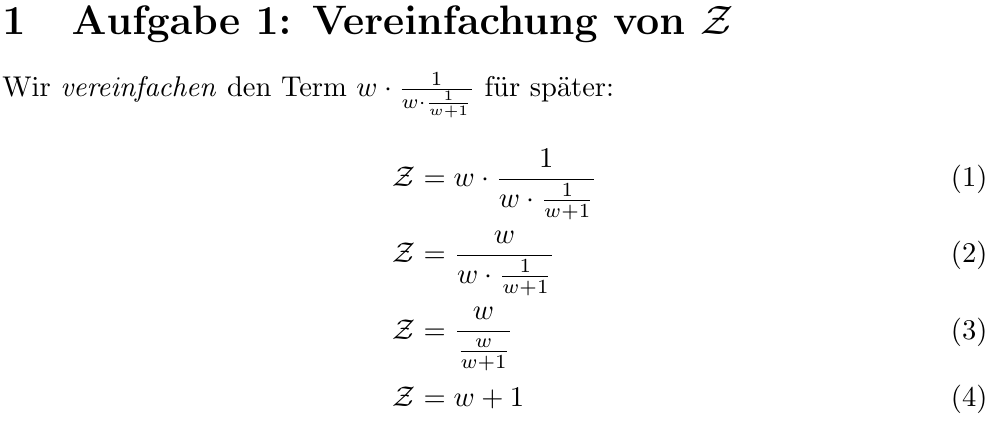
\includegraphics[width=0.95\textwidth]{images/mathe-uebung-1}
			\end{center}
		\end{frame}
			
		%%%%%%%%%%%%%%%%%%%%%%%%%%%%%%%%%%%%%%%%%%%%%%%%%%%%%%%%%%%%%%%%%%%%%%%
		
		\begin{frame}[containsverbatim]{Finale Übung}
			\slideheading{\LaTeX{}-Code:}\\
			{\footnotesize
			\begin{latexcode}
\section{Aufgabe 1: Vereinfacung von \(\mathcal{Z}\)}
Wir \textit{vereinfachen} den Term
\(w\cdot\frac{1}{w\cdot\frac{1}{w+1}}\) für später:
\begin{align}
	\mathcal{Z} &= w\cdot\frac{1}{w\cdot\frac{1}{w+1}}           \\
	\mathcal{Z} &=       \frac{w}{w\cdot\frac{1}{w+1}}\label{foo}\\
	\mathcal{Z} &=       \frac{w}{      \frac{w}{w+1}}           \\
	\mathcal{Z} &= w+1
\end{align}
Schritt \textbf{\ref{foo}} ist sehr wichtig.
			\end{latexcode}
			}
		\end{frame}
			
		%%%%%%%%%%%%%%%%%%%%%%%%%%%%%%%%%%%%%%%%%%%%%%%%%%%%%%%%%%%%%%%%%%%%%%%
		
	\section*{}
		\begin{frame}
			\begin{center}
				
\includegraphics[height=0.95\textheight]{./images/hotline}
			\end{center}
		\end{frame}
\end{document}

		\section{\LaTeX Advanced}
		\subsection{Referenzieren}
		
		%%%%%%%%%%%%%%%%%%%%%%%%%%%%%%%%%%%%%%%%%%%%%%%%%%%%%%%%%%%%%%%%%%%%%%%
		
		\begin{frame}[containsverbatim]{Referenzieren (Abschnitte)}
			\slideheading{\LaTeX-Code:}
			\begin{latexcode}
\subsection{Cliquen in bipartiten Graphen}
\label{sec:cliques}

% Irgendwo anders
Im Abschnitt \ref{sec:cliques} auf Seite
\pageref{sec:cliques} wurde das Finden von
Cliquen in bipartiten Graphen beschrieben.
			\end{latexcode}
			
			\slideheading{Ergebnis:}
			Im Abschnitt 3.2 auf Seite 7 wurde das Finden
			von Cliquen in bipartiten Graphen beschrieben.
		\end{frame}
		
		%%%%%%%%%%%%%%%%%%%%%%%%%%%%%%%%%%%%%%%%%%%%%%%%%%%%%%%%%%%%%%%%%%%%%%%
		
		\begin{frame}[containsverbatim]{Referenzieren (Figures)}
			\slideheading{\LaTeX-Code:}
			\begin{latexcode}
\begin{figure}[t]
	\includegraphics[width=7cm]{images/lichtstrahl}
	\caption{Brechung eines Lichtstrahls beim Wechsel
			 des Mediums}
	\label{fig:lichtbrechung}
\end{figure}
% Irgendwo anders
Der Lichtstrahl wird gebrochen, wie
Abbildung \ref{fig:lichtbrechung} zeigt.
			\end{latexcode}
			
			\slideheading{Ergebnis:}
			Der Lichtstrahl wird gebrochen, wie Abbildung 3 zeigt.
		\end{frame}
		
		%%%%%%%%%%%%%%%%%%%%%%%%%%%%%%%%%%%%%%%%%%%%%%%%%%%%%%%%%%%%%%%%%%%%%%%
		
		\subsection{Richtig Zitieren}
		
		\begin{frame}[containsverbatim]{Bib\TeX}
			\begin{itemize}
				\item Man verwaltet eine Bib\TeX{}-Datei (\texttt{*.bib}) mit Literaturangaben
				\item Mit \texttt{\textbackslash{}cite[Seite X]\{Referenz\}} referenziert man eine solche Angabe, mit optionaler Seitenangabe.
				\item Vor \texttt{pdflatex} wirft man \texttt{bibtex} an
			\end{itemize}
		\end{frame}
		
		%%%%%%%%%%%%%%%%%%%%%%%%%%%%%%%%%%%%%%%%%%%%%%%%%%%%%%%%%%%%%%%%%%%%%%%
		
		\begin{frame}[containsverbatim]{Bib\TeX}
			\slideheading{\LaTeX{}-Code:}
			\begin{latexcode}
% Im Header
\bibliographystyle{alpha}

% Beim Zitat
Für die Lösung des Travelling-Salesman-Problems
wurde ein heuristischer Algorithmus \cite{lin19973}
gewählt.

% An der Stelle des Literaturverzeichnis
\bibliography{literatur}
			\end{latexcode}
		\end{frame}
		
		%%%%%%%%%%%%%%%%%%%%%%%%%%%%%%%%%%%%%%%%%%%%%%%%%%%%%%%%%%%%%%%%%%%%%%%
		
		\begin{frame}[containsverbatim]{Bib\TeX-Eintrag}
			\slideheading{Bib\TeX{}-Eintrag:} (aus ``literatur.bib'')
			\begin{latexcode}
@article{lin1973,
	author  = {Shen Lin and Brian W. Kernighan},
	title   = {An Effective Heuristic Algorithm for the
	           Travelling-Salesman Problem},
	journal = {Operations Research},
	volume  = {21},
	year    = {1973},
	pages   = {498--516},
}
			\end{latexcode}
		\end{frame}
		
		%%%%%%%%%%%%%%%%%%%%%%%%%%%%%%%%%%%%%%%%%%%%%%%%%%%%%%%%%%%%%%%%%%%%%%%
		
		\begin{frame}{Bib\TeX{}-Ergebnis}
			\slideheading{Ergebnis:}
			
			% Das hier ist ist wieder ein wenig geschummelt um ein
			% Ergebnis, wie es in echten Dokumenten aussieht zu
			% emulieren. Das geht sicherlich auch hübscher.
			\vspace{0.2cm}
			Für die Lösung des Travelling-Salesman-Problems
			wurde ein heuristischer Algorithmus [LK73]
			gewählt.
			
			\vspace{0.5cm}
			{\Large \textbf{Literatur}}\\
			
			\vspace{0.3cm}
			\begin{tabular}{lp{9cm}}
				[LK73] & Shen Lin and Brian~W. Kernighan. An effective heuristic algorithm for
				         the travelling-salesman problem.
				         {\em Operations Research}, 21:498--516, 1973.
			\end{tabular}
		\end{frame}
		
		\subsection{Code-Highlighten}
		
		%%%%%%%%%%%%%%%%%%%%%%%%%%%%%%%%%%%%%%%%%%%%%%%%%%%%%%%%%%%%%%%%%%%%%%%
		
		\begin{frame}[containsverbatim]{Mit \texttt{minted}}
			\begin{itemize}
				\item \texttt{minted} arbeitet mit Pygments (python-library).
				\item Benötigt \texttt{-shell-escape} als Parameter von \texttt{pdflatex}. 
			\end{itemize}
			
			\slideheading{\LaTeX-Code:}
			\begin{latexcode}
\usepackage{minted}
% ...
\begin{minted}{java}
class MeineKlasse{
	private int meineVariable; // Deklaration
	
	public void meineMethode(){
		meineVariable = 42; // Initialisierung
	}
}
\end{minted}
			\end{latexcode}
		\end{frame}
		
		%%%%%%%%%%%%%%%%%%%%%%%%%%%%%%%%%%%%%%%%%%%%%%%%%%%%%%%%%%%%%%%%%%%%%%%
		
		\begin{frame}[containsverbatim]{Mit \texttt{minted}}
			\slideheading{Ergebnis:}
			\begin{minted}{java}
class MeineKlasse{
	private int meineVariable; // Deklaration
	
	public void meineMethode(){
		meineVariable = 42; // Initialisierung
	}
}
			\end{minted}
		\end{frame}
		
		%%%%%%%%%%%%%%%%%%%%%%%%%%%%%%%%%%%%%%%%%%%%%%%%%%%%%%%%%%%%%%%%%%%%%%%
		
		\begin{frame}[containsverbatim]{Mit \texttt{lstlisting}}
			\slideheading{\LaTeX-Code:}
			\begin{latexcode}
\usepackage{listings}
\lstset{...} % style-einstellungen
% ...
\begin{lstlisting}[caption=Variablen]
class MeineKlasse{
	private int meineVariable; // Deklaration
	
	public void meineMethode(){
		meineVariable = 42; // Initialisierung
	}
}
\end{lstlisting}
			\end{latexcode}
		\end{frame}
		
		%%%%%%%%%%%%%%%%%%%%%%%%%%%%%%%%%%%%%%%%%%%%%%%%%%%%%%%%%%%%%%%%%%%%%%%
		
		\begin{frame}[containsverbatim]{Mit \texttt{lstlisting}}
			\slideheading{Ergebnis:}
			\begin{lstlisting}[caption=Variablen]
class MeineKlasse{
	private int meineVariable; // Deklaration
	
	public void meineMethode(){
		meineVariable = 42; // Initialisierung
	}
}
			\end{lstlisting}
		\end{frame}
		
		%%%%%%%%%%%%%%%%%%%%%%%%%%%%%%%%%%%%%%%%%%%%%%%%%%%%%%%%%%%%%%%%%%%%%%%
		
		\subsection{Makros}
		\begin{frame}[containsverbatim]{Eigene Befehle}
			\slideheading{\LaTeX-Code:}
			\begin{latexcode}
% TeX-style
\def\heute{Heute ist der \today.}
% LaTeX-style (besser)
\newcommand{\heute}{Heute ist der \today.}
\newcommand{\TikZ}{Ti\textit{k}Z}
% Verwendung
\heute
\TikZ
			\end{latexcode}
			\slideheading{Ergebnis:}
			Heute ist der \today.\\
			\TikZ
		\end{frame}
		
		%%%%%%%%%%%%%%%%%%%%%%%%%%%%%%%%%%%%%%%%%%%%%%%%%%%%%%%%%%%%%%%%%%%%%%%
		
		\begin{frame}[containsverbatim]{Eigene Befehle}
			\slideheading{\LaTeX-Code:}
			\begin{latexcode}
% LaTeX-style
\newcommand{\bus}[4]{Ein Bus der Linie #1 Richtung 
                    #2 fährt von der Haltestelle
                    #3 um #4 ab.}
% Verwendung
\bus{181}{Sternschanze}{Informatikum}{13:37}
			\end{latexcode}
			\slideheading{Ergebnis:}
			\bus{181}{Sternschanze}{Informatikum}{13:37}
		\end{frame}
		
		%%%%%%%%%%%%%%%%%%%%%%%%%%%%%%%%%%%%%%%%%%%%%%%%%%%%%%%%%%%%%%%%%%%%%%%
		
		\begin{frame}[containsverbatim]{Eigene Umgebungen}
			\slideheading{\LaTeX-Code:}
			\begin{latexcode}
\newenvironment{textttit}
               {\begingroup\ttfamily\itshape}
               {\endgroup}
% Verwendung
\begin{textttit}
	Dies ist ein Test
\end{textttit}
			\end{latexcode}
			\slideheading{Ergebnis:}
			\texttt{\textit{Dies ist ein Test}}
		\end{frame}
		
		%%%%%%%%%%%%%%%%%%%%%%%%%%%%%%%%%%%%%%%%%%%%%%%%%%%%%%%%%%%%%%%%%%%%%%%
		
%		\section{HA-Tipps}
%		
%		\begin{frame}[containsverbatim]{\LaTeX{}-Beamer}
%			\begin{center}
%				Und jetzt ein paar Tipps für Hausaufgaben/-arbeiten
%			\end{center}
%		\end{frame}

		%%%%%%%%%%%%%%%%%%%%%%%%%%%%%%%%%%%%%%%%%%%%%%%%%%%%%%%%%%%%%%%%%%%%%%%

		\section{\protect\TikZ}
		
		\begin{frame}[containsverbatim]{\TikZ}
			\begin{itemize}
				\item \textbf{T}ikZ \textbf{i}st \textbf{k}ein \textbf{Z}eichenprogramm.
				\item Abbildungen werden mit TikZ beschrieben und durch PGF gerendert.
				\item Sehr umfangreiches Paket (Dokumentation: $>$1000 Seiten), viele Möglichkeiten.
				\item Hat direkte Unterstützung für Petrinetze :-)
				\item Overkill: Animationen in einer PDF mittels\\
				JavaScript und \TikZ ~:o
			\end{itemize}
			
			
			\vspace{-1.25cm}
			\hspace{8.5cm}
			\begin{tikzpicture}
				\draw[thick,rounded corners=8pt]
				(0,0) -- (0,2) -- (1,3.25) -- (2,2) -- 
				(2,0) -- (0,2) -- (2,2) -- (0,0) -- (2,0);
			\end{tikzpicture}
		\end{frame}

		%%%%%%%%%%%%%%%%%%%%%%%%%%%%%%%%%%%%%%%%%%%%%%%%%%%%%%%%%%%%%%%%%%%%%%%
		
		\subsection{Grundlagen}

		\begin{frame}[containsverbatim]{\TikZ}
			\begin{columns}[t]
				\column{0.7\textwidth}
				\slideheading{\LaTeX{}-Code:}
				\begin{latexcode}
\begin{tikzpicture}
	\draw[thick,rounded corners=8pt]
		(0,0) -- (0,2) -- (1,3.25) --
		(2,2) -- (2,0) -- (0,2) --
		(2,2) -- (0,0) -- (2,0);
\end{tikzpicture}
				\end{latexcode}
				
				\column{0.3\textwidth}
				\hspace{3mm}
				\slideheading{Ergebnis:}
				\hspace{3mm}
				\begin{tikzpicture}
					\draw[thick,rounded corners=8pt]
					(0,0) -- (0,2) -- (1,3.25) -- (2,2) -- 
					(2,0) -- (0,2) -- (2,2) -- (0,0) -- (2,0);
				\end{tikzpicture}
			\end{columns}
		\end{frame}

		%%%%%%%%%%%%%%%%%%%%%%%%%%%%%%%%%%%%%%%%%%%%%%%%%%%%%%%%%%%%%%%%%%%%%%%

		\begin{frame}[containsverbatim]{Nodes und Lines}
			\slideheading{\TikZ-Code:}
			\begin{latexcode}
\begin{tikzpicture}
	\node[shape=rectangle,draw=black,rounded corners]
		(s) at (0, 0) {S};
	\node[shape=rectangle,draw=black,rounded corners]
		(t) at (3, 0) {T};
	
	\draw[thick, ->]     (s)     -- (1, -1);
	\draw[thick, dotted] 
		(1, -1) to [bend right = 45] (2, -1);
	\draw[thick,->]      (2, -1) -- (t);
\end{tikzpicture}
			\end{latexcode}
		\end{frame}

		%%%%%%%%%%%%%%%%%%%%%%%%%%%%%%%%%%%%%%%%%%%%%%%%%%%%%%%%%%%%%%%%%%%%%%%

		\begin{frame}[containsverbatim]{Nodes und Lines}
			\begin{center}
				\slideheading{Ergebnis:}
				\vspace{0.5cm}
				\begin{tikzpicture}
					\node[shape=rectangle,draw=black,rounded corners]
						(s) at (0, 0) {S};
					\node[shape=rectangle,draw=black,rounded corners]
						(t) at (3, 0) {T};
					
					\draw[thick, ->]     (s)     -- (1, -1);
					\draw[thick, dotted] 
						(1, -1) to [bend right = 45] (2, -1);
					\draw[thick,->]      (2, -1) -- (t);
				\end{tikzpicture}
			\end{center}
		\end{frame}

		%%%%%%%%%%%%%%%%%%%%%%%%%%%%%%%%%%%%%%%%%%%%%%%%%%%%%%%%%%%%%%%%%%%%%%%

		\begin{frame}[containsverbatim]{Hobby-Kurven}
			\begin{itemize}
				\item Hobby-Kurven mittels \texttt{hobby}-Paket
			\end{itemize}
			\slideheading{\TikZ-Code:}
			\begin{smalllatexcode}
\begin{tikzpicture}
	\node[shape=rectangle,draw=black,rounded corners]
		(s) at (0, 0) {S};
	\node[shape=rectangle,draw=black,rounded corners]
		(t) at (3, 0) {T};
	
	\draw[thick, ->]     (s)     -- (1, -1);
	\draw[thick, ->, dotted] 
		(1, -1)
		to[curve through={(1.5, -1.1) .. (1.5,-0.75) .. (1.5, -1.1)}]
		(2, -1);
	\draw[thick, ->]      (2, -1) -- (t);
\end{tikzpicture}
			\end{smalllatexcode}
		\end{frame}

		%%%%%%%%%%%%%%%%%%%%%%%%%%%%%%%%%%%%%%%%%%%%%%%%%%%%%%%%%%%%%%%%%%%%%%%

		\begin{frame}[containsverbatim]{Hobby-Kurven}
			\begin{center}
				\slideheading{Ergebnis:}
				\vspace{0.5cm}
				\begin{tikzpicture}
					\node[shape=rectangle,draw=black,rounded corners] (s) at (0, 0) {S};
					\node[shape=rectangle,draw=black,rounded corners] (t) at (3, 0) {T};
					
					\draw[thick, ->]     (s)     -- (1, -1);
					\draw[thick, ->, dotted] 
 						(1, -1) 
 						to[curve through={(1.5, -1.1) .. (1.5,-0.75) .. (1.5, -1.1)}]
 						(2, -1);
					\draw[thick, ->]      (2, -1) -- (t);
				\end{tikzpicture}
			\end{center}
		\end{frame}

		%%%%%%%%%%%%%%%%%%%%%%%%%%%%%%%%%%%%%%%%%%%%%%%%%%%%%%%%%%%%%%%%%%%%%%%

		\begin{frame}[containsverbatim]{Styles für gesamtes \TikZ picture}
			\slideheading{\TikZ-Code:}
			\begin{smalllatexcode}
\begin{tikzpicture}
	[
		->,
		thick,
		knoten/.style={shape=rectangle,draw=black,rounded corners}
	]
	\node[knoten] (s) at (0, 0) {S};
	\node[knoten] (t) at (3, 0) {T};
	
	\draw (s)     -- (1, -1);
	\draw[dotted] 
		(1, -1) 
		to[curve through={(1.5, -1.1) .. (1.5,-0.75) .. (1.5, -1.1)}]
		(2, -1);
	\draw (2, -1) -- (t);
\end{tikzpicture}
			\end{smalllatexcode}
		\end{frame}

		%%%%%%%%%%%%%%%%%%%%%%%%%%%%%%%%%%%%%%%%%%%%%%%%%%%%%%%%%%%%%%%%%%%%%%%

		\begin{frame}[containsverbatim]{Styles für gesamtes \TikZ picture}
			\begin{center}
				\slideheading{Ergebnis:}
				\vspace{0.5cm}
				\begin{tikzpicture}
					[
						->,
						thick,
						knoten/.style={shape=rectangle,draw=black,rounded corners}
					]
					\node[knoten] (s) at (0, 0) {S};
					\node[knoten] (t) at (3, 0) {T};
					
					\draw (s)     -- (1, -1);
					\draw[dotted] 
 						(1, -1) 
 						to[curve through={(1.5, -1.1) .. (1.5,-0.75) .. (1.5, -1.1)}]
 						(2, -1);
					\draw (2, -1) -- (t);
				\end{tikzpicture}
			\end{center}
		\end{frame}

		%%%%%%%%%%%%%%%%%%%%%%%%%%%%%%%%%%%%%%%%%%%%%%%%%%%%%%%%%%%%%%%%%%%%%%%
		
		\subsection{Automaten}

		\begin{frame}[containsverbatim]{Einführung}
			\begin{itemize}
				\item Automaten (state-machines) per \texttt{automata}-Paket
				\item Für Positionierung \texttt{positioning}-Paket
				\item Und für Pfeile \texttt{arrows}-Paket
			\end{itemize}
			Mehr Informationen über Automaten, Pfeile, Positionierung, Optionen, etc. gibt es unter \href{http://hauke-stieler.de/public/tikz-for-state-machines.pdf}{http://hauke-stieler.de/public/tikz-for-state-machines.pdf} (im selben Ordner ist auch die \texttt{*.tex} Datei).
		\end{frame}

		%%%%%%%%%%%%%%%%%%%%%%%%%%%%%%%%%%%%%%%%%%%%%%%%%%%%%%%%%%%%%%%%%%%%%%%

		\begin{frame}[containsverbatim]{Zustände}
			\slideheading{\TikZ-Code:}
			\begin{latexcode}
\usetikzlibrary{
	automata,
	arrows}
% ...
\begin{tikzpicture}[->,
	>=stealth',
	semithick]
	
	\node[state,initial]   (0)              {$z_0$};
	\node[state]           (1) [right of=0] {$z_1$};
	\node[state,accepting] (2) [right of=1] {$z_2$};
\end{tikzpicture}
			\end{latexcode}
		\end{frame}

		%%%%%%%%%%%%%%%%%%%%%%%%%%%%%%%%%%%%%%%%%%%%%%%%%%%%%%%%%%%%%%%%%%%%%%%

		\begin{frame}[containsverbatim]{Zustände}
			\begin{center}
				\slideheading{Ergebnis:}
				\vspace{0.5cm}
				\begin{tikzpicture}[->,
					>=stealth',
					semithick]
					
					\node[state,initial]   (0)              {$z_0$};
					\node[state]           (1) [right of=0] {$z_1$};
					\node[state,accepting] (2) [right of=1] {$z_2$};
				\end{tikzpicture}
			\end{center}
		\end{frame}

		%%%%%%%%%%%%%%%%%%%%%%%%%%%%%%%%%%%%%%%%%%%%%%%%%%%%%%%%%%%%%%%%%%%%%%%

		\begin{frame}[containsverbatim]{Positionierung}
			\slideheading{\TikZ-Code:}
			\begin{smallerlatexcode}
\usetikzlibrary{
	automata,
	arrows,
	positioning}
% ...
\begin{tikzpicture}[->,
	>=stealth',
	semithick,
	node distance=2cm]
	
	\node [state] (a)                                {$a$};
	\node [state] (b) [above right=1cm and 2cm of a] {$b$};
	\node [state] (c) [below right of = a]           {$c$};
\end{tikzpicture}
			\end{smallerlatexcode}
		\end{frame}

		%%%%%%%%%%%%%%%%%%%%%%%%%%%%%%%%%%%%%%%%%%%%%%%%%%%%%%%%%%%%%%%%%%%%%%%

		\begin{frame}[containsverbatim]{Positionierung}
			\begin{center}
				\slideheading{Ergebnis:}
				\vspace{0.5cm}
				\begin{tikzpicture}[->,
					>=stealth',
					semithick,
					node distance=2cm]
					
					\node [state] (a)                                {$a$};
					\node [state] (b) [above right=1cm and 2cm of a] {$b$};
					\node [state] (c) [below right of = a]           {$c$};
				\end{tikzpicture}
			\end{center}
		\end{frame}

		%%%%%%%%%%%%%%%%%%%%%%%%%%%%%%%%%%%%%%%%%%%%%%%%%%%%%%%%%%%%%%%%%%%%%%%

		\begin{frame}[containsverbatim]{Pfeile}
			\slideheading{\TikZ-Code:}
			\begin{smalllatexcode}
\begin{tikzpicture}[->,
	>=stealth',
	semithick,
	node distance=2cm]

	\node [state,initial]   (a)            {$a$};
	\node [state]           (b)
		[above right=1cm and 2cm of a]     {$b$};
	\node [state,accepting] (c)
		[below right = 1cm and 1.5cm of a] {$c$};

	\path (a) edge node {0} (b)
	          edge node {1} (c)
	      (c) edge node {2} (b);
\end{tikzpicture}
			\end{smalllatexcode}
		\end{frame}

		%%%%%%%%%%%%%%%%%%%%%%%%%%%%%%%%%%%%%%%%%%%%%%%%%%%%%%%%%%%%%%%%%%%%%%%

		\begin{frame}[containsverbatim]{Pfeile}
			\begin{center}
				\slideheading{Ergebnis:}
				\vspace{0.5cm}
				\begin{tikzpicture}[->,
					>=stealth',
					semithick,
					node distance=2cm]
		
					\node [state,initial]   (a)            {$a$};
					\node [state]           (b)
						[above right=1cm and 2cm of a]     {$b$};
					\node [state,accepting] (c)
						[below right = 1cm and 1.5cm of a] {$c$};
				
					\path (a) edge node {0} (b)
					          edge node {1} (c)
					      (c) edge node {2} (b);
				\end{tikzpicture}
			\end{center}
		\end{frame}

		%%%%%%%%%%%%%%%%%%%%%%%%%%%%%%%%%%%%%%%%%%%%%%%%%%%%%%%%%%%%%%%%%%%%%%%

		\begin{frame}[containsverbatim]{Pfeile}
			\slideheading{\TikZ-Code:}
			\begin{smalllatexcode}
\begin{tikzpicture}[->,
	>=stealth',
	semithick,
	node distance=2cm]

	\node [state,initial]   (a)            {$a$};
	\node [state]           (b)
		[above right=1cm and 2cm of a]     {$b$};
	\node [state,accepting] (c)
		[below right = 1cm and 1.5cm of a] {$c$};

	\path (a) edge[above] node {0} (b)
	          edge[below] node {1} (c)
	      (c) edge[right] node {2} (b);
\end{tikzpicture}
			\end{smalllatexcode}
		\end{frame}

		%%%%%%%%%%%%%%%%%%%%%%%%%%%%%%%%%%%%%%%%%%%%%%%%%%%%%%%%%%%%%%%%%%%%%%%

		\begin{frame}[containsverbatim]{Pfeile}
			\begin{center}
				\slideheading{Ergebnis:}
				\vspace{0.5cm}
				\begin{tikzpicture}[->,
					>=stealth',
					semithick,
					node distance=2cm]
		
					\node [state,initial]   (a)            {$a$};
					\node [state]           (b)
						[above right=1cm and 2cm of a]     {$b$};
					\node [state,accepting] (c)
						[below right = 1cm and 1.5cm of a] {$c$};
				
					\path (a) edge[above] node {0} (b)
					          edge[below] node {1} (c)
					      (c) edge[right] node {2} (b);
				\end{tikzpicture}
			\end{center}
		\end{frame}

		%%%%%%%%%%%%%%%%%%%%%%%%%%%%%%%%%%%%%%%%%%%%%%%%%%%%%%%%%%%%%%%%%%%%%%%

		\begin{frame}[containsverbatim]{Pfeile}
			\slideheading{\TikZ-Code:}
			\begin{smalllatexcode}
\begin{tikzpicture}[->,>=stealth',
	shorten >=5pt,
	node distance=2.5cm,
	semithick]

	\node[initial,state]   (R)              {$z_r$};
	\node[state]           (S) [right of=R] {$z_s$};
	\node[state,accepting] (E) [right of=S] {$z_e$};
	
	\path   (R) edge [loop,above]       node {0}   (R)
				edge [below]            node {1}   (S)
		    (S) edge [loop,above]       node {0,1} (S)
				edge [below]            node {1}   (E)
		    (E) edge [bend left,below]  node {0}   (R)
				edge [loop,above]       node {0,1} (E);
\end{tikzpicture}
			\end{smalllatexcode}
		\end{frame}

		%%%%%%%%%%%%%%%%%%%%%%%%%%%%%%%%%%%%%%%%%%%%%%%%%%%%%%%%%%%%%%%%%%%%%%%

		\begin{frame}[containsverbatim]{Pfeile}
			\begin{center}
				\slideheading{Ergebnis:}
				\vspace{0.5cm}
				\begin{tikzpicture}[->,>=stealth',
					shorten >=5pt,
					node distance=2.5cm,
					semithick]
			
					\node[initial,state]   (R)              {$z_r$};
					\node[state]           (S) [right of=R] {$z_s$};
					\node[state,accepting] (E) [right of=S] {$z_e$};
					
					\path 	(R)	edge [loop,above]       node {0} (R)
								edge [below]            node {1} (S)
							(S)	edge [loop,above]       node {0,1} (S)
								edge [below]            node {1} (E)
							(E)	edge [bend left,below]  node {0} (R)
								edge [loop,above]       node {0,1} (E);
				\end{tikzpicture}
			\end{center}
		\end{frame}

		%%%%%%%%%%%%%%%%%%%%%%%%%%%%%%%%%%%%%%%%%%%%%%%%%%%%%%%%%%%%%%%%%%%%%%%

		\subsection{Funktionen Zeichnen}
		
		\begin{frame}[containsverbatim]{\TikZ}
			\begin{smalllatexcode}
\usepackage{pgf}
% ...
\begin{tikzpicture}[>=latex,semithick,font=\scriptsize,scale=0.75]
	\draw[very thin,color=lightgray] (-3.2,-1.2) grid (3.2,4.2);
	\draw[->] (-3.2,0) -- (3.4,0) node[right] {$x$};
	\draw[->] (0,-1.2) -- (0,4.4) node[above] {$y$};
    
	\foreach \x/\xtext in {-3/-3, -2/-2, -1/-1, 1/1, 2/2, 3/3}
	\draw[shift={(\x,0)}] (0pt,2pt) -- (0pt,-2pt) node[below] {$\xtext$};
	
	\foreach \y/\ytext in {-1/-1, 1/1, 2/2, 3/3, 4/4}
	\draw[shift={(0,\y)}] (2pt,0pt) -- (-2pt,0pt) node[left] {$\ytext$};
    
	\draw[thin,domain=-2.075:2.075,smooth,variable=\x,black]
		plot ({\x},{\x*\x});
	\draw[thin] node[inner sep=1mm,
					fill=white,
					draw=lightgray] at (2.25,3) {$f(x)=x^2$};
\end{tikzpicture}
			\end{smalllatexcode}
		\end{frame}

		%%%%%%%%%%%%%%%%%%%%%%%%%%%%%%%%%%%%%%%%%%%%%%%%%%%%%%%%%%%%%%%%%%%%%%%

		\begin{frame}{\TikZ}
			\begin{center}
				\slideheading{Ergebnis:}
				\begin{tikzpicture}[>=latex,semithick,font=\scriptsize,scale=0.75]
					\draw[very thin,color=lightgray] (-3.2,-1.2) grid (3.2,4.2);
				    
					\draw[->] (-3.2,0) -- (3.4,0) node[right] {$x$};
					\draw[->] (0,-1.2) -- (0,4.4) node[above] {$y$};
				    
					\foreach \x/\xtext in {-3/-3, -2/-2, -1/-1, 1/1, 2/2, 3/3}
					\draw[shift={(\x,0)}] (0pt,2pt) -- (0pt,-2pt) node[below] {$\xtext$};
				    
					\foreach \y/\ytext in {-1/-1, 1/1, 2/2, 3/3, 4/4}
					\draw[shift={(0,\y)}] (2pt,0pt) -- (-2pt,0pt) node[left] {$\ytext$};
				    
					\draw[thin,domain=-2.075:2.075,smooth,variable=\x,black]
						plot ({\x},{\x*\x});
					\draw[thin] node[inner sep=1mm,
									fill=white,
									draw=lightgray] at (2.25,3) {$f(x)=x^2$};
				\end{tikzpicture}
			\end{center}
		\end{frame}

		%%%%%%%%%%%%%%%%%%%%%%%%%%%%%%%%%%%%%%%%%%%%%%%%%%%%%%%%%%%%%%%%%%%%%%%

		\begin{frame}[containsverbatim]{Banyan-Netz (3 Stufen)}
			\begin{center}
				\vspace{-1.5cm}
				\hspace{-1.5cm}
				\begin{tikzpicture}
				[
					scale = 0.75,
					transform shape
				]
					\banyan{3}
				\end{tikzpicture}
			\end{center}
		\end{frame}

		%%%%%%%%%%%%%%%%%%%%%%%%%%%%%%%%%%%%%%%%%%%%%%%%%%%%%%%%%%%%%%%%%%%%%%%

		\begin{frame}[containsverbatim]{Banyan-Netz (5 Stufen)}
			\begin{center}
				\vspace{-0.5cm}
				\hspace{-1cm}
				\begin{tikzpicture}
				[
					scale = 0.19,
					transform shape
				]
					\banyan{5}
				\end{tikzpicture}
			\end{center}
		\end{frame}

		%%%%%%%%%%%%%%%%%%%%%%%%%%%%%%%%%%%%%%%%%%%%%%%%%%%%%%%%%%%%%%%%%%%%%%%

		\begin{frame}[containsverbatim]{5-dimensionaler Hyperwürfel}
			\begin{center}
				\begin{tikzpicture}
				[
					scale = 0.5,
					transform shape,
				]
					\hypercube
				\end{tikzpicture}
			\end{center}
		\end{frame}

		%%%%%%%%%%%%%%%%%%%%%%%%%%%%%%%%%%%%%%%%%%%%%%%%%%%%%%%%%%%%%%%%%%%%%%%

		\begin{frame}[containsverbatim]{}
			\begin{center}
				... mehrere kaputte Kaffeemaschinen später ...
			\end{center}
		\end{frame}

		%%%%%%%%%%%%%%%%%%%%%%%%%%%%%%%%%%%%%%%%%%%%%%%%%%%%%%%%%%%%%%%%%%%%%%%

		\begin{frame}[containsverbatim]{\TikZ at its best}
			\begin{center}
				\begin{tikzpicture}[scale=0.6,
				        %Option for nice arrows%
				        >=latex,%
				        inner sep=0pt,%
				        outer sep=2pt,%
				        mark coordinate/.style={outer sep=0pt,
				            minimum size=3pt, fill=black,circle}%
				    ]
				    %% some definitions
				    \def\R{0.5}       % sphere radius
				    \def\angEl{30}    % elevation angle
				    \def\angAz{-140}  % azimuth angle
				    \def\angPhi{-105} % longitude of point
				    \def\angBeta{55}  % latitude of point
				    \def\angGam{-190} % longitude of point
				    %% working planes
				    \pgfmathsetmacro\H{\R*cos(\angEl)}          % Distance to north pole
				    \LongitudePlane[xzplane]{\angEl}{\angAz}    % x-axis plane
				    %
				    \coordinate (O) at (0,0);
				    %
				    \begin{scope}[rotate around={-11.1:(0,0)},
				        field line/.style={color=red, smooth,
				            variable=\t, samples at={0,-5,-10,...,-360}}
				    ]
				        \clip[rotate around={11.1:(0,0)}] (-7,5) rectangle (7,-5);
				
				        % Computes a point on a field line given r and t
				        \newcommand{\fieldlinecurve}[2]{%
				            {(pow(#1,2))*(3*cos(#2)+cos(3*#2))}, {(pow(#1,2))*(sin(#2)+sin(3*#2))}%
				        }
				
				        % Longitudinal plnaes
				        \foreach \u in {0,-40,...,-160}{
				            \LongitudePlane[{{\u}zplane}]{\angEl}{\u}
				            \foreach \r in {0.25,0.5,...,2.25} {
				                \draw[{{\u}zplane}, field line]
				                plot (\fieldlinecurve{\r}{\t});
				            }
				        }
				        \foreach \u in {-200,-240,...,-320}{
				            \LongitudePlane[{{\u}zplane}]{\angEl}{\u}
				            \foreach \r in {0.25,0.5,...,2.25}{
				            \draw[{{\u}zplane}, dashed, field line]
				                plot (\fieldlinecurve{\r}{\t});
				            }
				        }
				        % Drawing plane for the B-vectors
				        \LongitudePlane[bzplane]{\angEl}{0}
				            \foreach \r in {0.25,0.5,...,2.25}{
				            \draw[bzplane, thick, field line]
				                plot (\fieldlinecurve{\r}{\t});
				        }
				
				        \begin{scope}[bzplane, very thick, ->, >=stealth]
				            \draw (\fieldlinecurve{1.25}{-30}) -- +(-30:0.79cm)  node[right] {$\vec{B_{r}}$};
				            \draw (\fieldlinecurve{1.25}{-30}) -- +(60:0.68cm)   node[right] {$\vec{B_{\theta}}$};
				            \draw (\fieldlinecurve{1.25}{30})  -- +(-150:0.79cm) node[below] {$\vec{B_{r}}$};
				            \draw (\fieldlinecurve{1.25}{30})  -- +(120:0.68cm)  node[above] {$\vec{B_{\theta}}$};
				        \end{scope}
				        %
				        \begin{scope}[rotate around={11.1:(0,0)}]
				            \fill[ball color=white,opacity=0.3] (O) circle (\R); %3D lighting effect
				            \draw (O) circle (\R);
				            \DrawLongitudeCircle[\R]{\angAz}      % xzplane
				            \DrawLongitudeCircle[\R]{\angAz + 90} % vzplane
				            \DrawLatitudeCircle[\R]{0}            % equator
				            \DrawLatitudeCircle[\R]{70}           % Latitude 70
				            \DrawLatitudeCircle[\R]{-70}          % Latitude -70
				        \end{scope}
				        %
				        \coordinate[mark coordinate] (Sm) at (0, \H);
				        \coordinate[mark coordinate] (Nm) at (0,-\H);
				        \path[xzplane] (Nm) -- +(0,-0.75) coordinate (Nm1) node[below] {$\mathbf{N}_m$}
				                       (Sm) -- +(0,0.75)  coordinate (Sm1) node[above] {$\mathbf{S}_m$};
				        \draw[very thick, dashed]    (Sm) -- (Nm);
				        \draw[very thick]            (Sm1) -- (Sm);
				        \draw[very thick,->,>=latex'](Nm) -- (Nm1);
				    \end{scope}
				\end{tikzpicture}
			\end{center}
		\end{frame}
		
		%%%%%%%%%%%%%%%%%%%%%%%%%%%%%%%%%%%%%%%%%%%%%%%%%%%%%%%%%%%%%%%%%%%%%%%
		
%		\section{Beamer}
%		
%		\begin{frame}[containsverbatim]{\LaTeX{}-Beamer}
%			\begin{center}
%				Und jetzt \LaTeX-Beamer
%			\end{center}
%		\end{frame}
\end{document}